% "{'classe':('PSI'),'chapitre':'dyn_1d','type':('td'),'titre':'Véhicule TIM', 'source':'Florestan Mathurin','comp':('C1-05','C2-08','C2-09'),'corrige':True}"
%\setchapterimage{fig_00}
\chapter*{TD \arabic{cptTD} \\ 
Véhicule TIM -- \ifprof Corrigé \else Sujet \fi}

\addcontentsline{toc}{section}{TD \arabic{cptTD} : Véhicule TIM -- \ifprof Corrigé \else Sujet \fi}

\iflivret \stepcounter{cptTD} \else
\ifprof  \stepcounter{cptTD} \else \fi
\fi
\setcounter{question}{0}

\marginnote{Florestan Mathurin.}
\marginnote{
\UPSTIcompetence[2]{C1-05}
\UPSTIcompetence[2]{C2-08}
\UPSTIcompetence[2]{C2-09}
}

\begin{marginfigure}
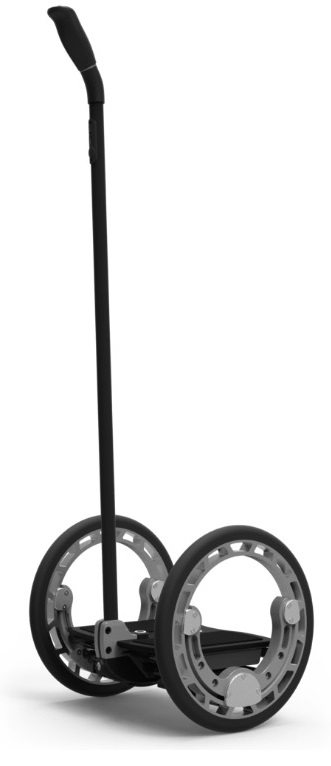
\includegraphics[width=\linewidth]{fig_01}
\end{marginfigure}


\ifprof
\else
L’éco-marathon SHELL est une compétition relative à la consommation énergétique des moyens de propulsion automobile. Les concurrents doivent concevoir et piloter leur véhicule sur une distance fixée avec une vitesse minimale imposée.  Les candidats sont ensuite classés en fonction de la consommation de leur véhicule, exprimée en «~kilomètre par litre~» de carburant. L’étude sur ce sujet, issue d’un projet élaboré par l’équipe T.I.M. de l’INSA Toulouse, a pour objet de quantifier les effets résistants et dissipatifs que sont la résistance au roulement et les actions aérodynamiques sur les performances de leur véhicule. Les effets inertiels étant plutôt quantifiés numériquement au niveau de la conception assistée par ordinateur du véhicule. 
\fi

\subsection*{Détermination expérimentale du coefficient de résistance au roulement}

\ifprof
\else


\begin{marginfigure}
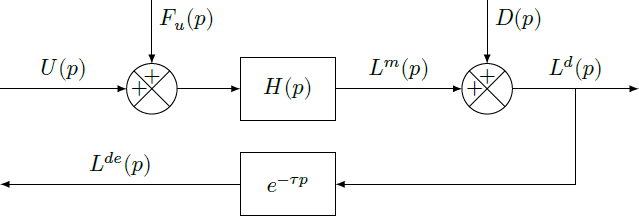
\includegraphics[width=\linewidth]{fig_02}
\end{marginfigure}

Le principe est présenté sur la figure 1. On place 2 roues lestées sur un dispositif inclinable. On considère ensuite que l’angle d’inclinaison minimum de la pente, où il y a début du mouvement des roues, est représentatif de la résistance au roulement.  
L’ensemble des 2 roues lestées peut être assimilé au solide \textbf{1} représenté sur la figure 1, de masse $m$, de rayon $R$ et de centre de masse $G$. 

L'accélération de la pesanteur $\vect{g}$ tel que $\vect{g}=-g\vect{z_0}$. 



L’action de contact entre l’ensemble des roues \sidenote{Cette action de contact peut s’écrire :$\torseurstat{T}{0}{1}=\torseurl{-T_{01}\vect{x}+N_{01}\vect{z}}{-C_r\vect{y}}{A_1}$ où $C_r$ représente le couple de résistance au roulement qui s’oppose au roulement tel que : $|C_r|=r|N_{01}|$ à la limite de l’équilibre et $|C_r|<r|N_{01}|$ à l’équilibre.} \textbf{1} et le plan \textbf{0}, incliné d’un angle $\alpha$ par rapport à l’horizontale, est  modélisé comme un contact ponctuel avec frottement où l’on tient compte de la résistance au roulement. 


%\subparagraph{}
%\textit{Réaliser un schéma illustrant les actions de contact. Préciser dans quel cas on se ici : limite du glissement sans roulement ou limite du roulement sans glissement ?}
\fi

\question{Écrire le principe fondamental de la statique appliqué au solide \textbf{1} réduit au point $G$ en projection sur la base $\base{x}{y}{z}$.}
\ifprof
\begin{corrige}
\begin{itemize}
\item On isole le solide 1. 
\item Le solide est soumis à l'action de pesanteur et à l'action du sol. 
\item On applique le PFS :
\begin{itemize}
\item TRS : $-T_{01}\vect{x}+N_{01}\vect{z}=-mg\vect{z_0}=-mg\left( \cos \alpha \vect{z}-\sin\alpha \vect{x} \right)$;
\item TMS en $G$ en projection sur $\vect{y}$: $-C_r+RT_{01}=0$.
\end{itemize}
\item On résout : 
\begin{itemize}
\item $-T_{01} +mg\sin\alpha = 0$;
\item $N_{01} -mg\cos\alpha = 0$;
\item $C_r=RT_{01}$.
\end{itemize}
\end{itemize}
%MG = MA1+GA1 ^ R
%MG = -Cry + z T01y   
\end{corrige}
\else
\fi


\question{Déterminer l’expression analytique de l’angle $\alpha_{\text{lim}}$ à la limite de l’équilibre quand il y a début du roulement du solide 1 sur le plan 0. }
\ifprof
\begin{corrige}
À la limite du roulement, on a $C_r=rN_{01}$ $\Leftrightarrow RT_{01}=rN_{01}$ $\Leftrightarrow Rmg\sin\alpha_{\text{lim}}=rmg\cos\alpha_{\text{lim}}$ et  $\tan \alpha_{\text{lim}} = \dfrac{r}{R}$.
\end{corrige}
\else
\fi

Pour une masse du solide 1 $m = \SI{50}{kg}$ et pour un rayon $R = \SI{0,25}{m}$ le roulement se produit à partir d’un angle  $\alpha_{\text{lim}}$ tel que $\tan \alpha_{\text{lim}} = 0,008$. 

\question{Déterminer le coefficient de résistance au roulement $r$.}
\ifprof
\begin{corrige}
$r=\SI{0,002}{m}$.
\end{corrige}
\else
\fi


\question{Au début du roulement, montrer qu’il ne peut pas y avoir glissement en $A_1$ si le coefficient de frottement au contact vaut $f = 0,5$. }
\ifprof
\begin{corrige}
À la limite du glissement, on a $T_{01}=fN_{01}$ et $\dfrac{T_{01}}{N_{01}}=\tan\alpha$. Pour $\tan \alpha_{\text{lim}}<f$ il y a donc roulement sans glissement. 
\end{corrige}
\else
\fi
\subsection*{Modélisation du véhicule}

\ifprof
\else

L’objectif est d’établir un modèle analytique du véhicule, lors d’une phase de roulement sans glissement sur une ligne droite inclinée d’un angle $\alpha$, en l’absence de vent. En adoptant des conditions particulières d’essai, il sera possible d’identifier précisément, grâce à ce modèle, les actions aérodynamiques. 

 Le modèle est donné figure suivante.
 
%\begin{marginfigure}
\marginnote{L’accélération de la pesanteur $\vect{g}$ telle que $\vect{g}=-g\vect{z_0}$.}

\begin{center}
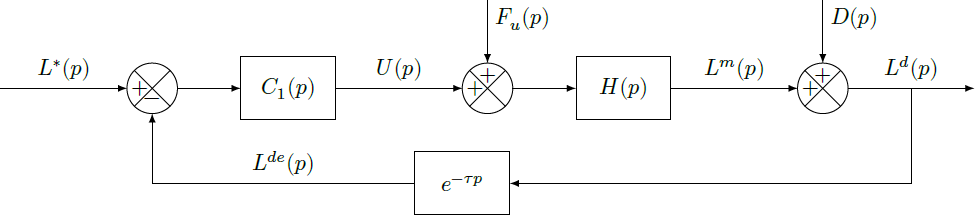
\includegraphics[width=.7 \linewidth]{fig_03}
\end{center}



\marginnote{Les roues sont en contact ponctuel avec frottement avec le sol 0. Afin de tenir compte de la résistance au roulement du pneu sur le sol, les actions de contact peuvent être modélisées en dynamique par : 
$\torseurstat{T}{0}{i}=\torseurl{-T_{0i}\vect{x}+N_{0i}\vect{z}}{-N_{0i}r\vect{y}}{A_i}$ avec $i=4$ ou 23.}

\marginnote{L’ensemble du véhicule dont la carrosserie est soumis lors de son mouvement à un effort de traînée aérodynamique qui peut être modélisée par le torseur 
$\torseurl{-\dfrac{1}{2}\rho S C_x \dot{x}^2 \vect{x}}{\vect{0}}{O_{23}}$ avec $\rho$ masse volumique du véhicule, $S$ surface alaire, $C_x$ coefficient de traînée du véhicule, $\dot{x}$ vitesse relative du véhicule par rapport à l'air ambiant. }

 On considère que le véhicule se déplace sur une pente inclinée d’un angle$\alpha$ par rapport à l’horizontale. Le véhicule est constitué :
\begin{itemize}
\item  d’un châssis avec son pilote : solide 1 de centre d’inertie $G$, de masse $M$ en translation par rapport au repère galiléen $R$ avec $\vect{OG}=x\vect{x}+R\vect{z}$;
\item de deux roues avant : solide 23 de centre d’inertie $O_{23}$, de masse $2 m$, de rayon $R$, dont le moment d’inertie par rapport à l’axe $\axe{O_{23}}{{y}}$ sera noté $2I$. Le solide 23 est en liaison pivot sans frottement par rapport au châssis 1 d’axe $\axe{O_{23}}{{y}}$ caractérisé par le paramètre $\theta_{23}$;
\item d’une roue arrière motrice : solide 4 de centre d’inertie $O_4$, de masse $m$, de rayon $R$, dont le moment d’inertie par rapport à l’axe $\axe{O_{4}}{{y}}$ sera noté $I$. Le solide 4 est en liaison pivot sans frottement par rapport au châssis 1 d’axe $\axe{O_{4}}{{y}}$ caractérisé par le paramètre $\theta_4$; 
\item un moteur d’entraînement du véhicule dont le corps est solidaire du châssis 1 exerce sur la roue 4 un couple moteur noté $C_m \vect{y}$. 
\end{itemize}





\fi

\question{Écrire les équations scalaires découlant des conditions de Roulement Sans Glissement (RSG) aux point $A_{23}$ et $A_4$.}
\ifprof
\begin{corrige}
En $A_{23}$, on a : $\vectv{A_{23}}{23}{0}=\vect{0}$. On a alors $\vectv{A_{23}}{23}{0}=\vectv{A_{23}}{23}{1}+\vectv{A_{23}}{1}{0}$ et $\vect{0}=\vectv{O_{23}}{23}{1}+\vect{A_{23}O_{23}}\wedge \vecto{23}{1}+\vectv{A_{23}}{1}{0} $ $\Leftrightarrow \vect{0}=\vect{0}+R\vect{z}\wedge \dot{\theta}_{23}\vect{y} + \dot{x}\vect{x}$ $\Rightarrow 0=-R \dot{\theta}_{23} + \dot{x}$.

De même en $A_4$, $0=-R \dot{\theta}_{4} + \dot{x}$.
\end{corrige}
\else
\fi

\question{En isolant l’ensemble $E=1+2+3+4$, écrire le théorème de la résultante dynamique en projection sur $\vect{x}$ et $\vect{z}$. }
\ifprof
\begin{corrige}
\begin{itemize}
\item On isole $E$.
\item BAME : 
\begin{itemize}
\item Pesanteur : $\torseurstat{T}{\text{Pes}}{E}=\torseurl{-\left(M+3m\right)g\vect{z_0}}{\vect{0}}{G_E}=\torseurl{-\left(M+3m\right)g\left( \cos \alpha \vect{z}-\sin \alpha \vect{x} \right)}{\vect{0}}{G_E}$.
\item Résistance au roulement : $\torseurstat{T}{T}{0}_i=\torseurl{-T_{0i}\vect{x}+N_{0i}\vect{z}}{-C_r\vect{y}}{A_i}$.
\item Traînée : $\torseurstat{T}{\text{Trainee}}{E}=\torseurl{-\dfrac{1}{2}\rho S C_x \dot{x}^2 \vect{x}}{\vect{0}}{O_{23}}$.
\end{itemize}
\item La résultante dynamique est donnée par $\left(M+3m\right)\vectg{G}{E}{0}=\left(M+3m\right)\ddot{x}\vect{x}$.
\item On applique le théorème de la résultante dynamique en projection sur $\vect{x}$ et $\vect{z}$ : 
\begin{itemize}
\item $\left(M+3m\right)g\sin \alpha -\dfrac{1}{2}\rho S C_x \dot{x}^2-T_{04}-T_{023}=\left(M+3m\right)\ddot{x}$
\item $-\left(M+3m\right)g \cos \alpha +N_{04}+N_{023}=0$
\end{itemize}
\end{itemize}
\end{corrige}
\else
\fi

\question{Pour chacune des roues 23 et 4, écrire les 2 équations scalaires correspondant au théorème du moment dynamique respectivement en $O_{23}$ et $O_4$ en projection sur $\vect{y}$. }
\ifprof
\begin{corrige}
\begin{itemize}
\item On isole 23. 
\item BAME : 
\begin{itemize}
\item 23 est soumis à la pesanteur;
\item action de la pivot sans frottement avec le solide 1;
\item résistance au roulement : $\torseurstat{T}{T}{0}_{23}=\torseurl{-T_{023}\vect{x}+N_{023}\vect{z}}{-N_{023}r\vect{y}}{A_{23}}=\torseurl{-T_{023}\vect{x}+N_{023}\vect{z}}{\left(-rN_{023}+RT_{023} \right)\vect{y}}{O_{23}}$.
\end{itemize}
\item Le moment dynamique de $O_{23}$ centre d'inertie des roues en projection sur $\vect{y_0}$ s'écrit $\vectmd{O_{23}}{23}{0}\vect{y_0}=2I\ddot{\theta}_{23}$.
\item TMD en $O_{23}$ en projection sur $\vect{y_0}$ s'écrit donc $-rN_{023}+RT_{023}=2I\ddot{\theta}_{23}$.
\end{itemize}
De même pour la roue 4 en ajoutant la sollicitation du couple moteur : 
$-rN_{04}+RT_{04}+C_m=I\ddot{\theta}_{4}$.
\end{corrige}
\else
\fi

\question{Montrer à partir des équations scalaires obtenues précédemment que le couple moteur $C_m$ vaut :
$C_m=\left( M+3m\right)g\cos\alpha r + \left[\dfrac{3I}{R}+R\left( M+3m\right) \right]\ddot{x}-R\left( M+3m\right)g\sin\alpha+\dfrac{1}{2}R\rho S C_x \dot{x}^2$. }
\ifprof
\begin{corrige}
On a :
%$-rN_{023}=-RT_{023}+2I\ddot{\theta}_{23}$x
%
%$R \dot{\theta}_{4} = \dot{x}$x
%$R \dot{\theta}_{23}= \dot{x}$x
%\begin{itemize}
%\item $\left(M+3m\right)g\sin \alpha -\dfrac{1}{2}\rho S C_x \dot{x}^2-\left(M+3m\right)\ddot{x}=T_{04}+T_{023}$
%\item x$ N_{04}=-N_{023}+\left(M+3m\right)g \cos \alpha$
%\end{itemize}
%
$C_m=I\ddot{\theta}_{4}+rN_{04}-RT_{04}$ $=\dfrac{I}{R}\ddot{x}+rN_{04}-RT_{04}$
$=\dfrac{I}{R}\ddot{x}-rN_{023}+r\left(M+3m\right)g \cos \alpha -RT_{04}$
$=\dfrac{I}{R}\ddot{x}-RT_{023}+2I\ddot{\theta}_{23}+r\left(M+3m\right)g \cos \alpha -RT_{04}$
$=\dfrac{I}{R}\ddot{x}+\dfrac{2I}{R}\ddot{x}+r\left(M+3m\right)g \cos \alpha -R\left(\left(M+3m\right)g\sin \alpha -\dfrac{1}{2}\rho S C_x \dot{x}^2-\left(M+3m\right)\ddot{x}\right)$. 

$C_m=r\left(M+3m\right)g \cos \alpha+\left(\dfrac{3I}{R}+R\left(M+3m\right)\right)\ddot{x} +\left(-R\left(M+3m\right)g\sin \alpha+ R\dfrac{1}{2}\rho S C_x \dot{x}^2\right)$. 

\begin{flushright}
\textit{CQFD.}
\end{flushright}

\end{corrige}
\else
\fi

\question{Identifier dans l’expression de $C_m$ les différentes actions qui ont tendance à affecter l’avancement du véhicule. }
\ifprof
\begin{corrige}

$$C_m=\underbrace{\left(M+3m\right)gr \cos \alpha}_{\text{Résistance au roulement}}-\underbrace{\left(M+3m\right)gR\sin \alpha}_{\text{Couple pour monter la pente}}+\underbrace{\left(\dfrac{3I}{R}+R\left(M+3m\right)\right)\ddot{x}}_{\text{Couple pour vaincre les effets d'inertie}} + \underbrace{R\dfrac{1}{2}\rho S C_x \dot{x}^2}_{\text{Couple pour vaincre la trainée}}$$. 

\end{corrige}
\else
\fi


\question{Déterminer l’expression du couple moteur $C_m$ quand le véhicule a une vitesse constante $V$ sur une piste horizontale. }
\ifprof
\begin{corrige}
À vitesse constante sur du plat, on a :
$$C_m=\underbrace{\left(M+3m\right)gr}_{\text{Résistance au roulement}} + \underbrace{R\dfrac{1}{2}\rho S C_x \dot{x}^2}_{\text{Couple pour vaincre la trainée}}$$. 
\end{corrige}
\else
\fi

\ifprof
\else

\begin{figure}[!h]
\centering
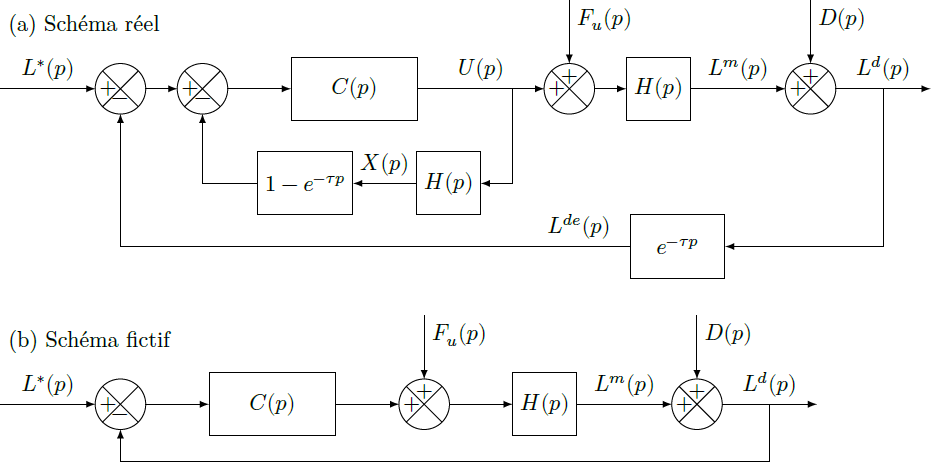
\includegraphics[width=.7\linewidth]{fig_04}
\end{figure}

On réalise un essai du véhicule sur terrain horizontal, le moteur du véhicule délivrant un couple $C_m$ constant.   
 L’acquisition des paramètres vitesse véhicule et distance parcourue sont visualisés par les graphes ci-contre. 

\marginnote{Les données véhicules sont :  $M = \SI{70}{kg}$, $m = \SI{1}{kg}$, $r = {2.10^{-3}}\text{m}$, $R = \SI{0,25}{m}$, $C_m= \SI{3,245}{m.N}$, $g = \SI{10}{ms^{-2}}$.}

\fi

\question{Déterminer dans les conditions d’essais le produit $\dfrac{1}{2}\rho S C_x$ caractérisant les effets aérodynamiques sur le véhicule. On précisera les unités. }
\ifprof
\begin{corrige}
La vitesse constante atteinte sur les graphes est de $\SI{17}{m.s^{-1}}$.  Par ailleurs 
$\dfrac{1}{2}\rho S C_x=\dfrac{C_m-\left(M+3m\right)gr}{R\dot{x}^2} =\dfrac{3,245-\left(70+3\cdot 1\right)\cdot 10 \cdot 0,002}{0,25\cdot 17^2}=\SI{0,025}{kg.m^{-1}}.$
\end{corrige}
\else
\fi


\question{Évaluer la pente maximum que peut monter ce véhicule à vitesse stabilisée de \SI{5}{km.h^{-1}} (on négligera le couple de résistance au roulement). }
\ifprof

\begin{corrige}
\end{corrige}
\else
\fi




\ifprof
\else
\begin{marginfigure}
\centering

\includegraphics[width=3cm]{Cy_01_Ch_03_TD_01_TIM_qr}
\end{marginfigure}
\fi


\ifprof
\else
\ifcolle
\else
%\marginnote{
\begin{solution}
\begin{enumerate}
\item $-T_{01} +mg\sin\alpha = 0$; $N_{01} -mg\cos\alpha = 0$; $C_r=RT_{01}$.
\item $\tan \alpha_{\text{lim}} = \dfrac{r}{R}$.
\item $r=\SI{0,002}{m}$.
\item Pour $\tan \alpha_{\text{lim}}<f$ il y a donc roulement sans glissement.
\item $\dot{x}=R \dot{\theta}_{23}$ et $\dot{x}=R \dot{\theta}_{4} $.
\item $\left(M+3m\right)g\sin \alpha -\dfrac{1}{2}\rho S C_x \dot{x}^2-T_{04}-T_{023}=\left(M+3m\right)\ddot{x}$ et $-\left(M+3m\right)g \cos \alpha +N_{04}+N_{023}=0$.
\item $-rN_{023}+RT_{023}=2I\ddot{\theta}_{23}$ et $-rN_{04}+RT_{04}+C_m=I\ddot{\theta}_{4}$.
\item $\,$
\item $\,$
\item $\,$
\item $\dfrac{1}{2}\rho S C_x = \SI{0,025}{kg.m^{-1}}$.
\item $\alpha=1\degres$.
\end{enumerate}
\end{solution}%}
\fi
\fi


